 \chapter{Polinômios}

\begin{obs}
  Um polinômio $p$ na incógnita $x$ e com coeficientes reais $\R$ é uma expressão da forma
\begin{equation*}
p(x)= a_nx^n + a_{n-1}x^{n-1}+ \ldots + a_1x+ a_0= \sum_{i=0}^{n} a_ix^i ,
\end{equation*}
  em que os coeficientes $a_n, \ldots, a_0 \in \R$, $a_n \neq 0$ e $n \in \N$. O número natural $n$ é chamado de grau do polinômio $p$, e escreve-se $gr(p)= n$. O termo $a_0$ é denominado termo constante de $p$.
\end{obs}

  Caso necessário, podemos tomar polinômios com coeficientes no conjunto dos números complexos $\C$.

 Os termos polinômio e função polinomial serão considerados como sinônimos e utilizados sem distinção no decorrer deste texto.

 Uma função polinomial de grau $0$ é uma função constante; uma função polinomial de grau $1$ é uma função linear (ou, função afim); uma função polinomial de grau $2$ é uma função quadrática.

 %Por simplicidade, a partir de agora iremos considerar nossos polinômios sobre $\R$, porém esta teoria pode ser estendida sem muita dificuldade para o corpo dos números complexos.

 \begin{obs}
 Dados um número real $k$ e o polinômio $p(x)= a_nx^n + a_{n-1}x^{n-1}+ \ldots + a_1x+ a_0$, chama-se \emph{valor numérico de $p$ em $k$} ao valor:
\begin{equation*}
p(k)= a_nk^n + a_{n-1}k^{n-1}+ \ldots + a_1k+ a_0 \ .
\end{equation*}
 \end{obs}

\begin{exem}
Se considerarmos o polinômio $p(x)= x^2 + 7x+10$, ele tem grau $2$ e temos os seguintes valores numéricos para $p$:
\begin{eqnarray*}
p(-6)&=& (-6)^2 + 7(-6) +10= 4\\
p(-5)&=& (-5)^2 + 7(-5) +10= 0\\
p(-4)&=& (-4)^2 + 7(-4) +10= -2\\
p(-2)&=& (-2)^2 + 7(-2) +10= 0\\
p(0)&=& 0^2 + 7 \cdot 0 +10= 10\\
\end{eqnarray*}
\end{exem}

 \begin{obs}
 Em particular, se $k$ é um número real tal que $p(k)= 0$, dizemos que $k$ é uma \emph{raiz} ou \emph{um zero} de $p$.
 \end{obs}

 \begin{exem}
 No caso $p(x)= x^2 + 7x+10$, temos que $k_1= -5$ e $k_2=-2$ são raízes do polinômio $p(x)= x^2 + 7x+10$.
 \end{exem}

  \begin{obs}
  O polinômio nulo (ou identicamente nulo) é um polinômio da forma cujos coeficientes são todos nulos, ou simplesmente, $p(x)= 0$. Por convenção, o grau deste polinômio será indefinido.
 \end{obs}


\begin{teo}
  Sejam $p$ e $q$ dois polinômios em $\R$, dados por:
\begin{align*}
p(x)&= a_nx^n + a_{n-1}x^{n-1}+ \ldots + a_1x+ a_0= \sum_{i=0}^{n} a_ix^i,\\
q(x)&= b_nx^n + b_{n-1}x^{n-1}+ \ldots + b_1x+ b_0= \sum_{i=0}^{n} b_ix^i.
\end{align*}
  
  Temos que $p=q$ se, e somente se, cada um dos coeficientes coincidem, isto é, $a_i= b_i$ para todo $i \in \{0, 1, 2, \cdots, n\}$.
 \end{teo}
 \begin{proof}
 Para todo $x \in \R$, temos:
\begin{gather*}
a_i= b_i \Leftrightarrow a_i - b_i=0 \Leftrightarrow (a_i - b_i)x^i=0 \Leftrightarrow \sum_{i=0}^{n}(a_i - b_i)x^i= 0 \Leftrightarrow\\
 \sum_{i=0}^{n}a_i x^i - \sum_{i=0}^{n}b_i x^i = 0 \Leftrightarrow \sum_{i=0}^{n}a_i x^i = \sum_{i=0}^{n}b_i x^i \Leftrightarrow p(x)= q(x).\qedhere
\end{gather*}
 \end{proof}

  Este teorema mostra que, quando escrevemos um polinômio $p$ na forma
\begin{equation*}
p(x)= a_nx^n + a_{n-1}x^{n-1}+ \ldots + a_1x+ a_0
\end{equation*}
 com $a_i \in \R$, então os números $a_0, \ldots, a_n$ são determinados de modo único.

\section{Operações com polinômios}

\subsection{Adição e subtração}
 Sejam $p$ e $q$ dois polinômios
\begin{align*}
p(x)&= a_nx^n + a_{n-1}x^{n-1}+ \ldots + a_1x+ a_0= \sum_{i=0}^{n} a_ix^i,\\
q(x)&= b_nx^n + b_{n-1}x^{n-1}+ \ldots + b_1x+ b_0= \sum_{i=0}^{n} b_ix^i
\end{align*}

A adição e subtração de polinômios é feita a partir da adição e subtração dos coeficientes correspondentes a um mesmo grau, ou seja,
\begin{align*}
(p+q)(x)&= (a_n+ b_n)x^n + (a_{n-1}+b_{n-1})x^{n-1}+ \ldots + (a_1+b_1)x+ (a_0+b_0)= \sum_{i=0}^{n} (a_i+b_i)x^i\\
(p-q)(x)&= (a_n- b_n)x^n + (a_{n-1}-b_{n-1})x^{n-1}+ \ldots + (a_1-b_1)x+ (a_0-b_0)= \sum_{i=0}^{n} (a_i-b_i)x^i.
\end{align*}

\begin{exem}
    Sejam $p(x)=2x^3-x^2+2$ e $q(x)=2x^5-7x^3+x-1$. Assim,
    \begin{align*}
        (p+q)(x)=2x^5-5x^3-x^2+x+1\\
        (p-q)(x)=-2x^5+9x^3-x^2-x+3.
    \end{align*}
\end{exem}

  \begin{prop}
  Se $p$, $q$ e $p+q$ são polinômios não nulos, então o grau do polinômio $p+q$ é menor ou igual ao maior dos números $gr(p)$ e $gr(q)$. Ou seja,
\begin{equation*}
gr(p+q) \leq \text{max}\{gr(p), gr(q)\} \ .
\end{equation*}
  \end{prop}

\subsection{Multiplicação}
A multiplicação entre polinômios é feita pela propriedade distributiva da multiplicação em relação à adição e multiplicação.

\begin{exem}
    Sejam $p(x)=2x-1$ e $q(x)=5x^2+2x-2$. Então,
    \begin{equation*}
        p(x)\cdot q(x)= (2x-1)(5x^2+2x-2) = 10x^3+4x^2-4x-5x^2-2x+2=10x^3-x^2-6x+2.
    \end{equation*}
\end{exem}

  \begin{prop}
  Se $p$, $q$ e $p \cdot q$ são polinômios não nulos, então o grau do polinômio $p \cdot q$ é igual a soma dos graus de $p$ e $q$;
\begin{equation*}
gr(p \cdot q) = gr(p) + gr(q) \ .
\end{equation*}
  \end{prop}

\subsection{Divisão}

Lembre que dividir um número inteiro $D$ (dividendo) por outro inteiro $d$ (divisor) diferente de zero consiste em encontrar dois números inteiros $q$ (quociente) e $r$ (resto), com $0\leqslant r<d$, tais que:
$D=qd+r$

Por exemplo, $7$ dividido por $2$ é $7=3\cdot 2 +1$, com quociente $3$ e resto $1$.

Da mesma forma, a divisão de um polinômio $p(x)$ por outro $d(x)$, com $d(x)\neq 0$, consiste em encontrar um par de polinômios $q(x)$ e $r(x)$ tais que satisfazem a equação
\begin{equation*}
    p(x)=q(x) d(x) +r(x)
\end{equation*}
em que $gr(r)<gr(d)$ ou $r(x)=0$. É garantido que sempre existe um único par de polinômios $q(x)$ e $r(x)$ com estas condições.

Chamamos de $p(x)$ o dividendo, $d(x)$ o  divisor, $q(x)$ o quociente e $r(x)$ o resto da divisão.

\begin{obs}
    A divisão é dita exata se $r(x)=0$. Neste caso, $p$ é divisível por $d$ ou $d$ é divisor de $p$.
\end{obs}

\begin{exem}
    A divisão do polinômio $p(x)$ por $x^2-3x$ resulta no quociente $x+2$ e resto $5$. Para descobrir $p(x)$ escrevemos
    \begin{equation*}
        p(x)=(x+2)(x^2-3x)+5 = x^3-3x^2+2x^2-6x+5=x^3-x^2-6x+5.
    \end{equation*}
\end{exem}

\begin{exem}
    Determine $m \ (m\neq 1)$ de modo que o polinômio $A(x)=(m-1)x^3-mx+2m+1$ seja divisível por $B(x)=x+1$.

    Veja que para ser divisível, o resto da divisão deve ser zero, isto é, $r(x)=0$. Como $m\neq 1$ então o dividendo tem grau 3, o divisor grau 1 e, portanto, o quociente tem grau 2. Denote por $q(x)=ax^2+bx+c$. Assim,
    \begin{equation*}
        (m-1)x^3-mx+2m+1 = (ax^2+bx+c)(x+1) = ax^3+(a+b)x^2+(b+c)x+c.
    \end{equation*}

    Igualando os coeficientes,
    \begin{equation*}
        \left\{
        \begin{matrix}
            a=m-1\\
            a+b=0\\
            b+c=-m\\
            c=2m+1
        \end{matrix}
        \right.
    \end{equation*}

    Assim, $b=-a=-m+1$ e $b=-m-c=-m-(2m+1)=-3m-1$. Portanto,
    \begin{gather*}
        -m+1=-3m-1\\
        3m-m=-1-1\\
        2m=-2\\
        m=-1.
    \end{gather*}
\end{exem}

\textbf{Método da chave:} Efetuar o a divisão pelo método da chave consiste em seguir os seguintes passos:
\begin{enumerate}
    \item Escreva os polinômios (dividendo e divisor) em ordem decrescente dos seus expoentes e completá-los, quando necessário, com termos de coeficiente zero.
    \item Dividir o termo de maior graus do dividendo pelo de maior grau do divisor, o resultado será um termo do quociente.
    \item Multiplicar o termo obtido no passo 2 pelo divisor e subtrair esse produto do dividendo;
    \item Se o grau da diferença for menor do que o do divisor, a diferença será o resto da divisão e o processo termina;
    \item Senão, retorne ao passo 2, considerando a diferença como um novo dividendo.
\end{enumerate}

\begin{exem}
    Encontre o quociente de $p(x)=2x^3 +3x-1$ por $d(x)=x^2+2x+5$.
    \begin{center}
    \polylongdiv[style=D]{2x^3 +3x-1}{x^2+2x+5}
    \end{center}
\end{exem}

\begin{exem}
    Encontre o quociente de $p(x)=x^3-4x^2+x+6$ por $d(x)=x+1$.
    \begin{center}
    \polylongdiv[style=D]{x^3-4x^2+x+6}{x+1}
    \end{center}
\end{exem}


\textbf{Dispositivo de Briott-Ruffini:} Este método é utilizado para calcular a divisão de um polinômio $p(x)$ por um polinômio de 1º grau da forma $x-a$. Como o grau do resto é sempre menor que o do divisor, então o resto deve ser um número $r\in\R$.

Este método será ilustrado pelo exemplo a seguir.

\begin{exem}
    Considere a divisão de $p(x)=3x^3-5x^2+x-2$ por $x-2$. Este método trabalha apenas com os coeficientes do polinômio $p(x)$ e com a raiz do divisor $x-2$, ou seja, o número $2$.

    \begin{enumerate}
        \item Colocamos a raiz do divisor seguida dos coeficientes do dividendo em ordem decrescente das potências de $x$. Repetimos o primeiro coeficiente do dividendo na linha de baixo.
        \begin{center}
            \polyhornerscheme[x=2,tutor=true,stage=2,tutorstyle=\color{red},showbase=top]{3x^3-5x^2+x-2}
        \end{center}

        \item  Multiplicamos a raiz do divisor pelo coeficiente repetido e adicionamos o produto com o segundo coeficiente, colocando o resultado abaixo dele.
        \begin{center}
            \polyhornerscheme[x=2,tutor=true,stage=4,tutorstyle=\color{red}, tutorlimit=2,showbase=top]{3x^3-5x^2+x-2}
        \end{center}

        \item Repetimos o processo anterior com os 3º e 4º coeficientes do dividendo, sucessivamente.
        \begin{center}
            \polyhornerscheme[x=2,tutor=true,stage=6,tutorstyle=\color{red}, tutorlimit=2,showbase=top]{3x^3-5x^2+x-2}
            \hspace{2cm}
            \polyhornerscheme[x=2,tutor=true,stage=8,tutorstyle=\color{red}, tutorlimit=2,showbase=top]{3x^3-5x^2+x-2}
        \end{center}

        \item O último número obtido é o resto da divisão e os outros números à esquerda são os coeficientes do quociente.
        \begin{center}
            \polyhornerscheme[x=2,resultbottomrule,resultleftrule,resultrightrule,showbase=top,showmiddlerow=false]{3x^3-5x^2+x-2}
        \end{center}
    \end{enumerate}
    
    Logo, $q(x)=3x^2+x+3$ e o resto é $r=4$.
\end{exem}

\begin{exem}
    Vamos determine o resto da divisão de $x^6-1$ por $x+1$. Pelo dispositivo de Briott-Rufini
    \begin{center}
            \polyhornerscheme[x=-1,resultbottomrule,resultleftrule,resultrightrule,showbase=top,showmiddlerow=false,equalcolwidths=true]{x^6-1}
        \end{center}

    Assim, o resto da divisão é zero.
\end{exem}

\section{Teorema do Resto}

\begin{teo}[Teorema do Resto]
    O resto da divisão de um polinômio $p(x)$ por um binômio $x-a$ é igual ao valor numérico de $p(x)$ em $x=a$, isto é, $p(a)=r$.
\end{teo}
\begin{proof}
    Como o grau do resto é sempre menor que o do divisor, então o resto deve ser um número $r\in\R$. Assim, $p(x)=(x-a)q(x)+r$ e
    \begin{equation*}
        p(a)=(a-a)q(a)+r=0\cdot q(a)+r=r.\qedhere
    \end{equation*}
\end{proof}

\begin{teo}[Teorema de D'Alembert]
    Um polinômio $p(x)$ é divisível por $x-a$ se, e somente se, $p(a)=0$.
\end{teo}

\begin{exem}
    O polinômio $p(x)=x^3+4x^2+x-6$ é divisível por $x+2$ pois $p(-2)=(-2)^3+4(-2)^2-2-2=0$.
\end{exem}

% \todo[inline]{PAREI AQUI}
% ------------------

%   Para funções polinomiais o \emph{Teorema Fundamental da Álgebra} garante a existência de zeros.

%   \begin{teo}[Teorema Fundamental da Álgebra]
%   Seja $p \in \C[x]$ um polinômio não constante. Então existe um número complexo $z_0$ tal que $p(z_0)=0$.
%   \end{teo}

%   \begin{proof}
%   A demonstração deste resultado pode ser encontrada em livros de Cálculo de uma variável complexa ou Análise Complexa como por exemplo página 119 do (SOARES, 2009).
%   \end{proof}

%   Como consequência direta do Teorema Fundamental da Álgebra temos o seguinte teorema.

%   \begin{teo}
%   Todo polinômio de grau $n \geq 1$ possui pelo menos uma raiz real ou complexa.
%   \end{teo}

%  Observe que estes resultados garantem que todo polinômio possui pelo menos uma raiz complexa, como vamos focar nossos estudos em polinômios sobre $\R$, podemos neste caso ter polinômios que não possuem raízes reais. Ainda sobre as raízes de um polinômio vale destacar o seguinte teorema.

%  \begin{teo}
%   Seja $p$ um polinômio não nulo em $K$, escrito na forma
% \begin{equation*}
% p(x)= a_nx^n + a_{n-1}x^{n-1}+ \ldots + a_1x+ a_0
% \end{equation*}
%    então $p$ tem no máximo $n$ raízes em $K$.
%  \end{teo}

%  \begin{teo}
%   Sejam $p(x)$, $g(x)$ polinômios sobre o corpo $K$, i.e., polinômios em $K[x]$, e suponhamos que $gr(g) \geq 0$. Então, existem polinômios $q(x)$ e $r(x)$ tais que
% \begin{equation*}
% p(x)= q(x)g(x) + r(x) \ , 
% \end{equation*}
%   em que $gr(r) < gr (g)$. Essas condições permitem determinar os polinômio $q$ e $r$ de modo único.
%  \end{teo}

%  \begin{proof}
%  A demonstração deste teorema pode ser encontrada na página 58 do (LANG, 1972).
%  \end{proof}



%  \begin{exem}
%   Como um exemplo para a divisão de polinômios, façamos a divisão do polinômio $p_1(x)=x^3-4x^2+x+6$ pelo binômio $g_1(x)=x+1$:

%  \begin{figure}[H]
%  \centering
%  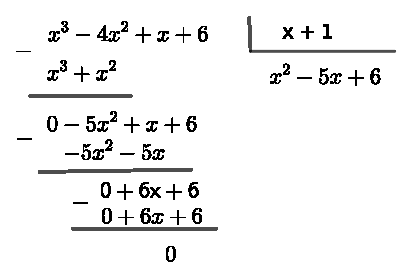
\includegraphics[width=8cm]{./cap_expralg/figs/polinomiosdivisao}
%  \end{figure}

%  note que o quociente da divisão é $q_1(x)= x^2 - 5x + 6$, e o resto desta divisão é $r(x)=0$ (zero). Como o resto é zero concluímos que $p_1(x)$ é divisível por $g_1(x)$. Portanto $p_1(x)= q_1(x)g_1(x)$, ou seja, $x^3-4x^2+x+6= (x^2-5x+6)(x+1)$.
%  \end{exem}

%  Como consequência do teorema anterior, temos o seguinte corolário, que nos garante que no exemplo anterior $-1$ é uma raiz do polinômio $p_1(x)$.

%  \begin{coro}
%  Seja $p$ um polinômio não-nulo sobre $K$. Seja $\alpha \in K$ tal que $p(\alpha)=0$. Então, existe um polinômio $q(x)$ sobre $K$ tal que
% \begin{equation*}
% p(x)= (x - \alpha)q(x) \ .
% \end{equation*}
%  \end{coro}

%  Como consequência deste Corolário, todo polinômio de grau $n \geq 1$ pode ser escrito como produto de $n$ fatores de grau $1$.

%  \begin{teo}[Teorema da Decomposição]
%   Todo polinômio $p(x)= a_nx^n + a_{n-1}x^{n-1}+ \ldots + a_1x+ a_0$, com $a_n \neq 0$, pode ser escrito de forma fatorada
% \begin{equation*}
% p(x)= a_n(x - r_1)(x - r_2) \ldots (x - r_n)
% \end{equation*}
%   onde $r_1, r_2, \cdots, r_n$ são as raízes do polinômio.
%  \end{teo}

\section{Equações polinomiais}

Dado um polinômio $p(x)$ de grau $n>0$, uma equação polinomial (ou algébrica) é uma equação da forma $p(x)=0$, ou seja, uma equação algébrica de grau $n$ é uma equações do tipo:
\begin{equation*}
    a_n x^n+a_{n-1} x^{n-1}+\cdots+ a_1 x+a_0=0.
\end{equation*}

O número $r$ é uma raiz da equação $p(x)=0$ se, e somente se, $p(r)=0$.

\begin{obs}
As equações algébricas de 1º e 2º grau já foram descritas. As equações de 3º grau possuem raízes descritas pelas fórmulas de Cardano; já as raízes das equações de 4º grau possuem raízes são obtidas pelas fórmulas de Ferrari.

As equações de grau superior a 4 não apresentam fórmulas resolutivas em termos dos coeficientes do polinômio.
\end{obs}

Ainda é possível que haja soluções para estas equações de grau 5 ou superior. Para funções polinomiais o \emph{Teorema Fundamental da Álgebra} garante a existência de zeros.

\begin{teo}[Teorema Fundamental da Álgebra]
Toda equação algébrica de grau $n$ admite um total de $n$ raízes complexas.
\end{teo}

Note que o teorema garante a existência de soluções complexas, mas não diz como obtê-las. Além disso, uma equação algébrica pode não possuir soluções reais.

\subsection{Multiplicidade de uma raiz e fatoração}

Dizemos que a equação $p(x)=0$ possui raiz $r$ de multiplicidade $m$, com $m\geqslant 1$, se, e somente se, podemos escrever
\begin{equation*}
    p(x)=(x-r)^m q(x) =0
\end{equation*}
tal que $q(r)\neq 0$. Ou seja, $p(x)$ é divisível por $(x-r)^m$.

\begin{exem}
    A equação $x^5\cdot (x+7)^3 = 0$ possui raízes $x=0$ com multiplicidade $5$ e $x=-7$ com multiplicidade 3.
\end{exem}

\begin{obs}
    Dado uma equação $p(x)=a_n x^n+a_{n-1} x^{n-1}+\cdots+ a_1 x+a_0=0$ de grau $n>0$ tal que $r_1,\dots,r_n$ são todas as raízes da equação (eventualmente com repetição quando a multiplicidade é maior que 1). Então, o polinômio $p(x)$ pode ser fatorado da forma:
    \begin{equation*}
        p(x)=a_n\cdot (x-r_1)\cdot (x-r_2) \cdots (x-r_n).
    \end{equation*}
\end{obs}

 \section{Equações racionais}

 \begin{obs}
  As equações racionais são dadas por quocientes/razões de polinômios da forma:
  \[\dfrac{p(x)}{q(x)}= 0\]
  onde $p(x)$ e $q(x)$ são polinômios na variável $x$ e $q(x) \neq 0$.
 \end{obs}
 
 Lembre-se que não podemos dividir por $0$ (zero), logo a equação racional
 \[\dfrac{p(x)}{q(x)}= 0\]
 está definida apenas no conjunto $D= \{x \in \R \mid q(x) \neq 0\}$.
 
 Este subconjunto dos números reais no qual a equação está bem definida é chamado de domínio da equação. A solução de uma equação racional é necessariamente um subconjunto do domínio da mesma.
 
 Vejamos alguns exemplos de como resolver uma equação racional.
 
 \begin{exem} $\dfrac{1}{x}= \dfrac{4}{3x} + 1$
 
 Para resolver esta equação começamos determinando seu domínio. Para isso lembremos que não existe divisão por $0$ (zero), logo um número real $x$ pertence ao domínio desta equação se, e somente se, 
 $x \neq 0$ e $3x \neq 0 \Rightarrow x \neq 0$.
 
 Portanto, o domínio desta equação é o conjunto
 \[D= \{ x \in \R \mid x \neq 0 \} \ . \]
 
 Agora vamos resolver a equação,
 \begin{eqnarray*}
 \dfrac{1}{x} = \dfrac{4}{3x} + 1.
 \end{eqnarray*}
 
 Precisamos tirar o MMC dos denominadores, pois os mesmos são diferentes
 \begin{eqnarray*}
 \dfrac{3}{3x}= \dfrac{4 + 3x}{3x} \\
 \dfrac{3-4-3x}{3x} = 0.
 \end{eqnarray*}
 
 Lembre que esta equação é zero somente quando o numerador for zero, logo basta olhar o numerador,
 \begin{eqnarray*}
 -1 = 3x \Rightarrow x= \dfrac{-1}{3}.
 \end{eqnarray*}
 
 Como $\frac{-1}{3} \in D$ decorre que o conjunto solução desta equação é $S= \left\{ \dfrac{-1}{3} \right\}$.
 \end{exem}
 
 % \begin{exem} $\dfrac{2x^2 - 6x}{x - x^3}= 0$
 
 % Calculando o domínio:
 % \begin{gather*}
 % x - x^3 \neq 0\\
 % x - x^3 = 0 \Leftrightarrow x(1-x^2)= 0 \Leftrightarrow x= 0 \text{ ou } x^2= 1 \Rightarrow x= \pm 1
 % \end{gather*}
 
 % Portanto, o domínio desta equação é o conjunto
 % \[D= \{ x \in \R \mid x \neq 0; x \neq 1; x \neq -1 \}= \R \setminus \{-1, 0, 1\}. \]
 
 % Agora vamos resolver a equação,
 % \begin{eqnarray*}
 % \dfrac{2x^2 - 6x}{x - x^3}= 0 \\
 % \dfrac{x(2x - 6)}{x(1 - x^2)}= 0 \\
 % \dfrac{2x - 6}{1 - x^2}= 0 \\
 % 2x - 6= 0 \\
 % x= 3.
 % \end{eqnarray*}
 
 % Como $3 \in D$ decorre que o conjunto solução desta equação é $S= \{ 3 \}$.
 % \end{exem}
 
 \begin{exem} $1 - \dfrac{2}{x}= \dfrac{8}{x^2}$
 
 Calculando o domínio. Um número real $x$ pertence ao domínio desta equação se:
 \begin{eqnarray*}
  x \neq 0 \text{ e } x^2 \neq 0 \Rightarrow x \neq 0
 \end{eqnarray*}
 
 Portanto, o domínio neste caso é
 \[D= \{ x \in \R \mid x \neq 0 \}= \R \setminus \{0\} \ . \]
 
 Agora vamos resolver a equação,
 \begin{eqnarray*}
 1 - \dfrac{2}{x}= \dfrac{8}{x^2} \\
 \dfrac{x^2}{x^2} - \dfrac{2x}{x^2}= \dfrac{8}{x^2} \\
 x^2 - 2x= 8 \\
 x^2 -2x -8= 0 \\
 (x-4)(x+2)= 0 \\
 x_1= 4 \text{ ou } x_2= -2.
 \end{eqnarray*}
 
 Como $\{-2, 4\} \subset D$ decorre que o conjunto solução desta equação é $S= \{ -2, 4 \}$.
 \end{exem}
 
 % \begin{exem} $\dfrac{x^3 -39x + 70}{x^2 + 2x - 8}= 0$
 
 % Calculando o domínio. 
 
 % Um número real $x$ pertence ao domínio desta equação se:
 % \begin{eqnarray}
 %  x^2 + 2x - 8 \neq 0 
 % \end{eqnarray}
 % como as raízes desta equação do 2º grau são $-4$ e $2$, decorre que o domínio neste caso é
 % \[D= \{ x \in \R \mid x \neq -4; x \neq 2 \}= \R \setminus \{-4, 2\} \ . \]
 
 % Vamos resolver a equação.
 
 % 1ª Forma: Note que a equação é satifeita quando o numerador for zero, logo basta resolver
 % \begin{eqnarray}
 % x^3 -39x + 70= 0 \\
 % (x+7)(x-2)(x-5)= 0 \\
 % x= -7 \text{ ou } x= 2 \text{ ou } x= 5
 % \end{eqnarray}
 
 % Agora precisamos verificar quais soluções da equação $x^3 -39x + 70= 0$ estão no conjunto $D$, note que $2 \notin D$ e $\{-7, 5\} \subset D$ portanto nosso conjunto solução é:
 % \[S= \{ -7, 5 \} \ . \]
 
 % 2º Forma: Podemos também proceder da seguinte forma:
 % \begin{eqnarray}
 % \dfrac{x^3 -39x + 70}{x^2 + 2x - 8}= 0 \\
 % \dfrac{(x+7)(x-2)(x-5)}{(x-2)(x+4)}= 0 \\
 % \dfrac{(x+7)(x-5)}{(x+4)}= 0 \\
 % (x+7)(x-5)= 0 \\
 % x= -7 \text{ ou } x= 5
 % \end{eqnarray}
 % Como $x= -7$ e $x= 5$ não são raízes de $x^2+2x-8=0$, e portanto pertecem ao domínio $D$, decorre que nosso conjunto solução é:
 %  \[S= \{ -7, 5 \} \ . \]
 % \end{exem}
 
  \begin{exem} $\dfrac{x^3 - 7x^2 + 16x -12}{x-2}=0 $
 
 Calculando o domínio. Um número real $x$ pertence ao domínio desta equação se:
 \begin{eqnarray*}
  x - 2 \neq 0  \Rightarrow x \neq 2
 \end{eqnarray*}
 
 Portanto, o domínio neste caso é
 \[D= \R \setminus \{2\} \ . \]
 
 Agora vamos resolver a equação, para isso vou escrever o polinômio de grau 3 na forma fatorada.
 \begin{eqnarray*}
 \dfrac{x^3 - 7x^2 + 16x -12}{x-2}=0 \\
 \dfrac{(x-2)(x-2)(x-3)}{x -2}=0 \\
 (x-2)(x-3)=0 \\
 x_1= 2 \text{ ou } x_2= 3.
 \end{eqnarray*}
 
 Como $2 \notin D$ e $3 \in D$ decorre que o conjunto solução desta equação é $S= \{ 3 \}$.
 
 Observe que neste caso mesmo após a simplicação da fração, uma das raízes da equação resultante não pertence ao domínio da nossa equação racional, pois ela é também raíz do polinômio presente no denominador da equação original, e por isso não pode fazer parte do conjunto solução procurado.
 \end{exem}


\newpage

\begin{secExercicios}

    \begin{exer}
    \item Determine quais expressões são polinômios:
    \begin{enumerate}[a)]
    \begin{multicols}{2}
         \item $3x^2+2x^4-7^{-2}$
         \item $x^{\frac{2}{5}}-5x+3$
         \item $(4x^2-1)^6$
         \item $(a+3)x^4+\sqrt{3}$
         \item $3x^{-3}+2x^{-2}$
         \item $3+\pi x$
         \item $x^{\sqrt{2}}+x$
         \item $x^x$
    \end{multicols}
    \end{enumerate}
    \end{exer}
    \begin{resp}
     a) Sim; b) Não; c) Sim; d) Sim; e) Não; f) Sim; g)Não; h) Não.
    \end{resp}

    \begin{exer}
        Seja o polinômio $p(x)=x^4-3x^2-5$. Calcule $p(-1)-\frac{1}{7}p(3)$.
    \end{exer}
    \begin{resp}
        $-14$.
    \end{resp}

        \begin{exer}
        Dados os polinômios $p(x)=10x^4-3x^2+3x+10$ e $q(x)=2x^2-5x$, calcule e dê o grau dos seguintes polinômios:
        \begin{enumerate}[a)]
        \begin{multicols}{2}
            \item $(p+q)(x)$
            \item $-3\cdot p(x)$
            \item $(p\cdot q)(x)$
            \item $p(x)-5x^2\cdot q(x)$
        \end{multicols}
        \end{enumerate}
    \end{exer}

    \begin{exer}
        Determine $a,b$ e $c$ de modo que $(a+b-1)x^2+(b-2c)x+(2c-1)=0$.
    \end{exer}
    \begin{resp}
        $a=0$, $b=1$, $c=\frac{1}{2}$.
    \end{resp}

    \begin{exer}
        O quociente da divisão de um polinômio $p(x)$ por $x^2+x+1$ é igual a $2x^3+3x^2-1$, e o resto da divisão é $11x-7$. Qual é o polinômio $p(x)$?
    \end{exer}

    \begin{exer}
        Efetue as seguintes divisões:
        \begin{enumerate}[a)]
            \item $x^5+3x^2-6x+8$ por $x+2$
            \item $4y^3-2y^2+5y-6$ por $y-1$
            \item $x^4-10x^3+24x^2+10x-24$ por $x^2-6x+5$
            \item $3x^4-x^2+4x$ por $x-2$
        \end{enumerate}
    \end{exer}

    \begin{exer}
        (ITA) A divisão de um polinômio $p(x)$ por $x^2-x$ resulta no quociente $6x^2+5x+3$ e resto $-7x$. Qual o resto da divisão de $p(x)$ por $2x+1$?
    \end{exer}

    \begin{exer}
        Determine o valor de $r$ no polinômio $p(x)=x^3+4x^2+rx-3$, sabendo que $-2$ é raiz.
    \end{exer}

    \begin{exer}
        Dado $p(x)=(m^2-1)x^2+(m-1)x+7$, descreva o grau deste polinômio em função de $m$.
    \end{exer}

    \begin{exer}
        (UnB) Seja $p(x)=x^3+4x^2+kx+(k-51)$. Determine o valor de $k$, sabendo que $p(x)$ é divisível por $x-1$.
    \end{exer}

    \begin{exer}
        Verifique se o polinômio $p(x)=2x^3+5x^2-x-6$ é divisível por $(x-1)(x-2)$.
    \end{exer}

    \begin{exer}
        Determine o polinômio $p(x)=ax^2+bx+c$ sabendo que $p(0)=5$, $p(1)=6$ e $p(-2)=-9$.
    \end{exer}
    \begin{resp}
        $p(x)=-2x^2+3x+5$.
    \end{resp}

    \begin{exer}
        Calcule as raízes de $p(x)=x^3-4x^2+9x-10$, sabendo que $p(x)$ é divisível por $x-2$.
    \end{exer}

    \begin{exer}
        O polinômio $p(x)= x^4+x^3-13x^2-25x -12$ possui somente raízes reais.  Encontre todas as raízes de $p(x)$ sabendo que este polinômio é divisível por $(x+1)^2$. Em seguida, fatore $p(x)$.
    \end{exer}
    
    \begin{exer}
    Considere o polinômio $p(x)=x^3 +r x^2 -4rx +6$, onde $r$ é um número real constante.
    \begin{enumerate}[a)]
        \item Determine o valor de $r$ de modo que $P(x)$ seja divisível por $x+6$.
        \item Usando o valor encontrado de $r$ no item (a), fatore o polinômio $p(x)$.
    \end{enumerate}
    \end{exer}
    
    \begin{exer}
        Dados os polinômios $p(x)=8x^5-5x^4+7x^3-3x+4$ e $q(x)=4x^2-5$, determine:
        \begin{multicols}{2}
            \begin{enumerate}[a)]
                \item $p(x+1)$
                \item $p(q(x))$
                \item $(p\cdot q)(x)$
                \item $\dfrac{-2 \cdot p(x)}{q(x)}$
                \item $\dfrac{p(x)}{x+2}$
            \end{enumerate}
        \end{multicols}
    \end{exer}
    \begin{resp}
%        \par\noindent\rule{\columnwidth}{0.4pt}
    \end{resp}

    \begin{exer}
    Resolva as seguintes equações racionais:
    
    \begin{multicols}{2}
    \begin{enumerate}[a)]
    \item $\dfrac{448}{7x}= \dfrac{144}{9x} + 8$
    \item $\dfrac{2x^2 - 2x}{x - x^3}= 0$
    \item $\dfrac{-1}{x}= \dfrac{-6}{x^2} + 1$
    \end{enumerate}
    \end{multicols}
    \end{exer}
    \begin{resp}
    \begin{multicols}{2}
     \begin{enumerate}[a)]
    \item $S= \{6 \}$
    \item $S= \varphi$
    \item $S= \{-3; 2\}$
    \end{enumerate}
    \end{multicols}
    %    \par\noindent\rule{\columnwidth}{0.4pt}
    \end{resp}

%\subsection*{Respostas:}

%\shipoutAnswer


\end{secExercicios}

%\section{Equações polinomiais e fatoração}

